\documentclass[border=6pt]{standalone}
\usepackage{tikz}
\usetikzlibrary{arrows.meta,positioning,shapes.geometric,shapes.multipart,calc,fit,backgrounds,decorations.pathreplacing,decorations.markings,automata,chains,matrix,patterns}
\usepackage{circuitikz}
\usepackage{amsmath}
\usepackage{amssymb}
\begin{document}
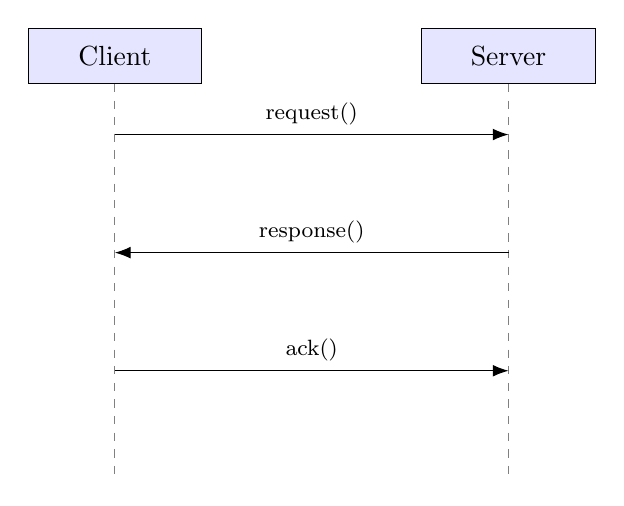
\begin{tikzpicture}[
  actor/.style={rectangle, draw, fill=blue!10, minimum width=2.2cm, minimum height=0.7cm},
  lifeline/.style={dashed, gray},
  msg/.style={-{Latex[length=2mm]}}
]
  \node[actor] (A) at (0,0) {Client};
  \node[actor] (B) at (5,0) {Server};
  \draw[lifeline] (A.south) -- ++(0,-5);
  \draw[lifeline] (B.south) -- ++(0,-5);

  \draw[msg] (0,-1) -- node[above, font=\footnotesize]{request()} (5,-1);
  \draw[msg] (5,-2.5) -- node[above, font=\footnotesize]{response()} (0,-2.5);
  \draw[msg] (0,-4) -- node[above, font=\footnotesize]{ack()} (5,-4);
\end{tikzpicture}
\end{document}
